\documentclass{standalone}
\usepackage{pgf, tikz}
\usetikzlibrary{arrows, automata, positioning}

\begin{document}

    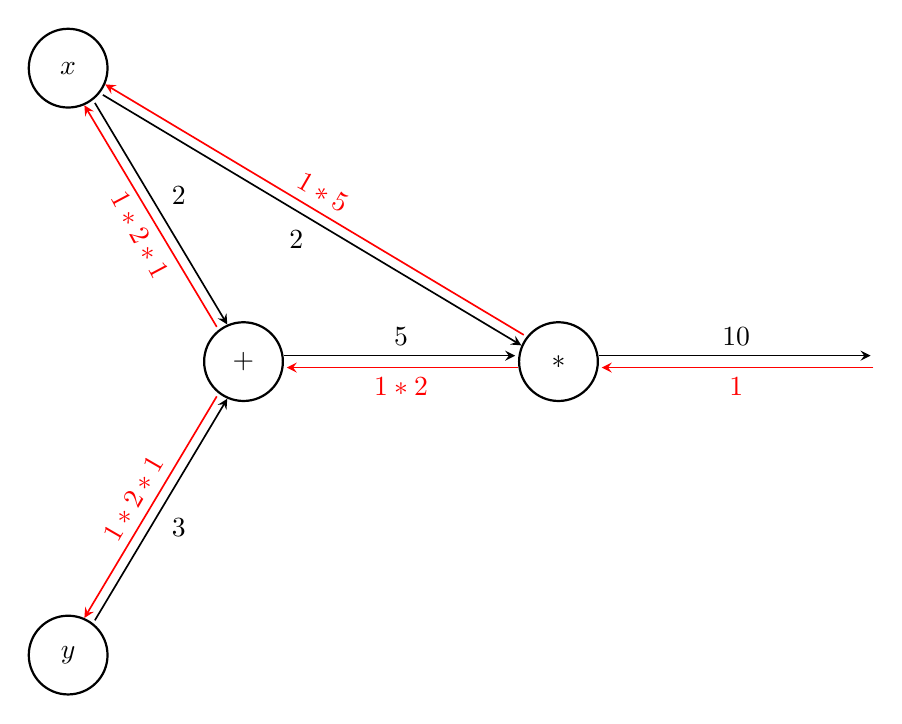
\begin{tikzpicture}[
            > = stealth, 
            shorten > = 1pt, 
            auto,
            node distance = 4cm,
            semithick
        ]

        \tikzstyle{every state}=[
            draw = black,
            thick,
            fill = white,
            minimum size = 10mm
        ]
        %\tikzset{every edge/.append style={font=\large}}

		\node[state] (add) {$+$};
        \node[state] (x) [above left=3cm and 1.5cm of add] {$x$};
        \node[state] (y) [below left=3cm and 1.5cm of add] {$y$};        
        \node[state] (mul) [right of=add] {$*$};
        \coordinate[right of=mul] (f);
        
        \path[->,transform canvas={xshift=0.5ex}] (x) edge node[above right] {$2$} (add);        
        \path[->,transform canvas={yshift=-0.5ex}] (x) edge node[below left] {$2$} (mul);        
        \path[->,transform canvas={xshift=0.5ex}] (y) edge node[below right] {$3$} (add);        
        \path[->,transform canvas={yshift=0.5ex}] (add) edge node {$5$} (mul);
        \path[->,transform canvas={yshift=0.5ex}] (mul) edge node {$10$} (f);
      
      
        \path[->,transform canvas={yshift=-0.5ex}] (f) edge[red] node {$1$} (mul);
        \path[->,transform canvas={yshift=0.5ex}] (mul) edge[red] node[above, rotate=-30] {$1*5$} (x);
        \path[->,transform canvas={yshift=-0.5ex}] (mul) edge[red] node {$1*2$} (add);
        \path[->,transform canvas={xshift=-0.5ex}] (add) edge[red] node[above, rotate=60] {$1*2*1$} (y);        
        \path[->,transform canvas={xshift=-0.5ex}] (add) edge[red] node[below, rotate=-62, pos=0.45] {$1*2*1$} (x);
        

    \end{tikzpicture}

\end{document}